% ::setlocal makeprg=cd\ latex\ &&\ pdflatex\ -interaction=batchmode\ main.tex\ &&\ xdg-open\ main.pdf\ &&\ exit

As we have seen in the previous chapter, the Schwarzschild metric describes the
geometry of spacetime around a spherically symmetric, non-rotating black hole.
Even though it is one of the simplest solutions to the Einstein field equations,
the orbits of particles, in general, are not described by closed form solutions.

In this chapter we will build a program in \texttt{C} that numerically
integrates the equations of motion.
The program will allow us to study more complex geodesics and better understand
how they differ from the Newtonian case.


\section{Equations of motion}
\label{cap2:sec:eq_of_motion}

Recalling the results of the previous chapter we can rewrite the equation for
the radial motion \ref{cap1:eq:like_newton}, together with the equations for
$\phi$ and $t$ that come directly from the conservation of angular momentum and
energy per rest mass unit, respectively eq. \ref{cap1:eq:conserved_l} and
\ref{cap1:eq:conserved_e}.

\begin{subequations}
\label{cap2:eq:eq_of_motion}
	\begin{align}[left = {\empheqlbrace}]
        &\frac{1}{2} \left(\dv{r}{\tau}\right)^2 = \mathcal E - V_{\rm eff} (r)
        \\
        &\dv{\phi}{\tau} = \frac{l}{r^2} \\
        &\dv{t}{\tau} = \frac{e}{1 - 2 M / r}
	\end{align}
\end{subequations}

Where $V_{\rm eff}$ is the effective potential defined in eq.
\ref{cap2:fig:V_eff} and $\mathcal E = \frac{e^2 - 1}{2}$.

To avoid numerical problems, we will keep geometrized units and express
everything in unit of the \Sh radius $r_s = 2 M$:

\begin{equation}
    r = r_s \hat r \quad \quad
    \tau = r_s \hat \tau \quad \quad
    t = r_s \hat t \quad \quad
    \ell = r_s \hat \ell \quad \quad
\end{equation}

The system of equations \ref{cap2:eq:eq_of_motion} can be rewritten as

\begin{subequations}
    \begin{align}[left = {\empheqlbrace}]
        &\dv{\hat r}{\hat \tau} = \pm \sqrt{2 \mathcal E - 2 V_{\rm eff}}
        \label{cap2:eq:radial_eq_as} \\
        &\dv{\phi}{\hat \tau} = \frac{\hat \ell}{\hat r^2}
        \label{cap2:eq:angular_eq_dimless} \\
        &\dv{t}{\hat \tau} = \sqrt{2 \mathcal E + 1}
        \left(\frac{\hat r}{\hat r - 1}\right) \label{cap2:eq:time_eq_dimless}
    \end{align}
    \label{cap2:eq:eq_of_motion_ad}
\end{subequations}

The effective potential becomes

\begin{equation}
    V_{\rm eff} = \frac{1}{2} \left(\frac{\hat \ell^2}{\hat r^2}
    - \frac{1}{\hat r} - \frac{\hat \ell^2}{\hat r^3} \right) \, .
    \label{cap2:eq:V_eff}
\end{equation}

The condition on the angular momentum $\ell$ for the existence of a stable
orbits is $\ell > \sqrt{12} M$ and becomes $\hat \ell > \sqrt{3}$.
The stationary points of $V_{\rm eff}$ from eq. \ref{cap1:eq:V_eff} are

\begin{subequations}
    \begin{align}
        \hat r_{\substack{\text{min} \\ \text{max}}} &= \hat \ell^2
        \left(1 \pm \sqrt{1 - \frac{3}{\hat \ell^2}} \right)
        &&{\rm for} \quad \hat \ell > \sqrt{3} \\
        \hat r_{\rm ISCO} &= 3
        &&{\rm for} \quad \hat \ell = \sqrt{3}
    \end{align}
\end{subequations}

Where $\hat r_{\substack{\text{min} \\ \text{max}}}$ respectively represent a
local minimum and maximum of the effective potential.
The system in \ref{cap2:eq:eq_of_motion_ad} can be solved numerically with
a fourth-order \texttt{Runge-Kutta} method.
The initial conditions that determine the orbit are $\hat \ell$,
$\mathcal E$ and a compatible starting radius $\hat r_0$ (refer to Figure
\ref{cap1:fig:V_eff_orbits}).

To find the range of $r$ that the particle can explore we need to study when the
argument of the square root in eq. \ref{cap2:eq:radial_eq_as} is positive.
In general, we need to solve a cubic equation

\begin{equation}
    \dv{\hat r}{\hat \tau} = 0
    \quad \Rightarrow \quad
    \mathcal E - V_{\rm eff} = 0
    \quad \Rightarrow \quad
    \hat r^3 - \hat \ell^2 \hat r^2 + \hat \ell^2 - 2 \mathcal E
    \hat r - \hat \ell^2 = 0 \, .
    \label{cap2:eq:cubic_eq}
\end{equation}

All the possible scenarios are resumed in Table \ref{cap2:tab:scenarios}.

\begin{table}[h]
    \centering
    \begin{tabular}{cccc}
        $\hat \ell$     & $\mathcal E$                  & $\hat r$     
                                                        & Scenario \\
        $[0,~\sqrt{3}]$ & $[0,~\infty]$                 & $(1,~\infty)$
                                                        & depends on the sign\\
        $[0,~\sqrt{3}]$ & $[-\frac{1}{2},~0]$           & $(1,~r_e)$   
                                                        & infall \\
        $(\sqrt{3},~2]$ & $[0,~\infty]$                 & $(1,~\infty)$ 
                                                        & depends on the sign \\
        $(\sqrt{3},~2]$ & $[V_{\rm max},~0]$            & $(1,~r_2)$
                                                        & infall \\
        $(\sqrt{3},~2]$ & $[V_{\rm min},~V_{\rm max}]$  & $(r_1,~r_2)$
                                                        & bound orbit \\
        $(\sqrt{3},~2]$ & $[-\frac{1}{2},~V_{\rm min}]$ & $(1,~r_e)$
                                                        & infall \\
        $(2, \infty)$   & $[V_{\rm max},~\infty]$       & $(1,~\infty)$ 
                                                        & depends on the sign \\
        $(2, \infty)$   & $[0,~V_{\rm max}]$            & $(r_1,~\infty)$
                                                        & unbound orbit \\
        $(2, \infty)$   & $[V_{\rm min},~V_{\rm min}]$  & $(r_1,~r_2)$
                                                        & bound orbit \\
        $(2, \infty)$   & $[-\frac{1}{2},~V_{\rm min}]$ & $(1,~r_e)$
                                                        & infall \\
    \end{tabular}
    \caption{Possible scenarios for the motion of a particle in the \Sh
    spacetime.}
    \label{cap2:tab:scenarios}
    %% A Figure would probably be better
\end{table}

In the table we referred to the local maximum and minimum of the effective
potential calculated in $r_{\substack{\text{min} \\ \text{max}}}$ as
$V_{\rm min}$ and $V_{\rm max}$ respectively.
Instead of solving the cubic equation analytically, the limiting radii can be
calculated using the bisect method and imposing that \ref{cap2:eq:cubic_eq}
must be 0 between 1 and $r_{\rm min}$ for $r_e$, between $r_{\rm min}$ and
$r_{\rm max}$ for $r_1$ and between $r_{\rm max}$ and $\infty$ (1000 in our
case) for $r_2$.

%% NON MI PIACE






\section{Numerical integration}

Similarly to the previous chapter, we can start with a radial infall scenario,
where $\hat \ell = 0$, $\mathcal E = 0$.

\begin{figure}[h]
    \begin{minipage}{0.48\textwidth}
        \centering
        \includegraphics[width=\textwidth]{Figures/chapter2/radial_infall_plot.eps}
        \caption{Plot of the orbit of a particle in radial infall ($\hat \ell = 0$
        and $\mathcal E = 0$). \\}
    \end{minipage}
    \hspace{0.015 \textwidth}
    \begin{minipage}{0.48\textwidth}
        \centering
        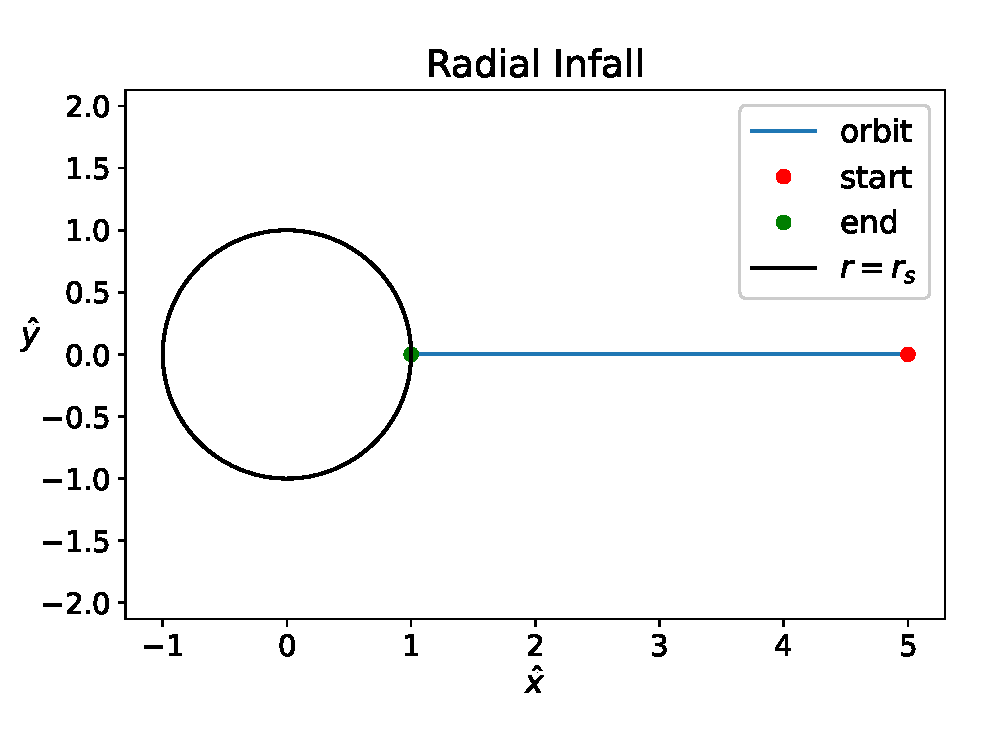
\includegraphics[width=\textwidth]{Figures/chapter2/radial_infall.eps}
        \caption{Proper time against \Sh time with respect of the radius of a
        particle falling towards $r = r_s$.}
    \end{minipage}
\end{figure}

The orbit plot is not the most interesting, but the time plot shows that the
numerical integration is working correctly, as the results are consistent with
eq. \ref{cap1:eq:radial_infall_r_of_tau} and \ref{cap1:eq:radial_infall_r_of_t}
found analytically in the previous chapter.

By integrating numerically with this program, we can visualize some more
complex infalls.

\begin{figure}[h]
    \begin{minipage}{0.48\textwidth}
        \centering
        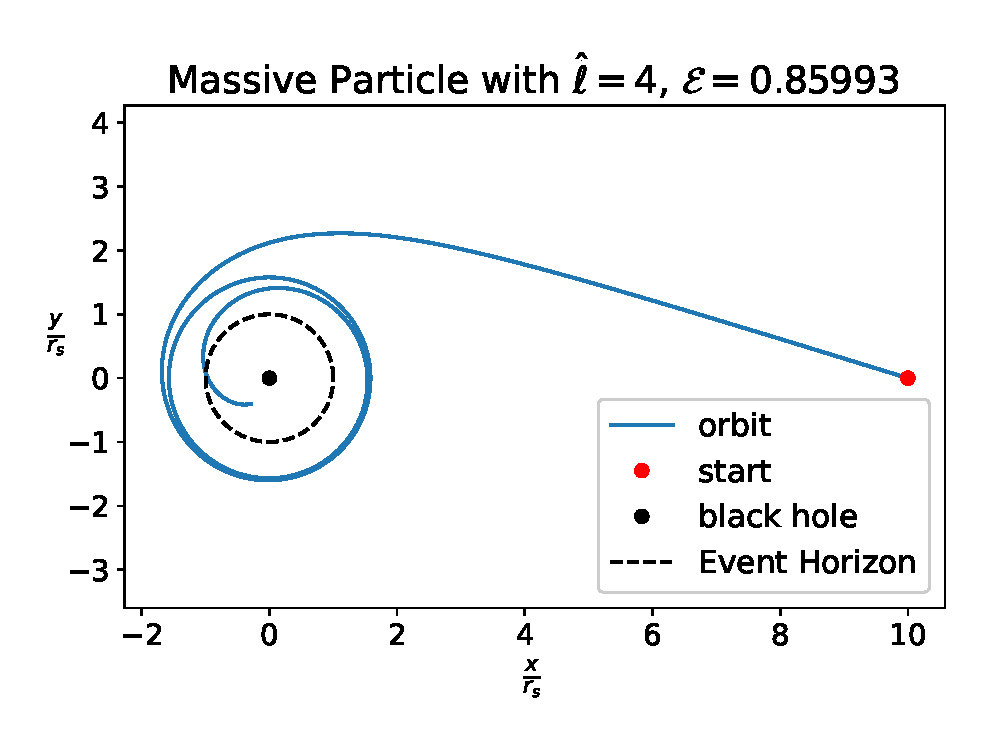
\includegraphics[width=\textwidth]{Figures/chapter2/infall1.eps}
        \caption{Plot of the orbit of a particle with $\hat \ell = 1$
        and $\mathcal E = 0.85993$.
        The energy was chosen to be slightly above $V_{\rm eff}(r_{\rm max})$ to
        decrease the radial velocity when approaching $\hat r = r_{\rm max}$.}
    \end{minipage}
    \hspace{0.015 \textwidth}
    \begin{minipage}{0.48\textwidth}
        \centering
        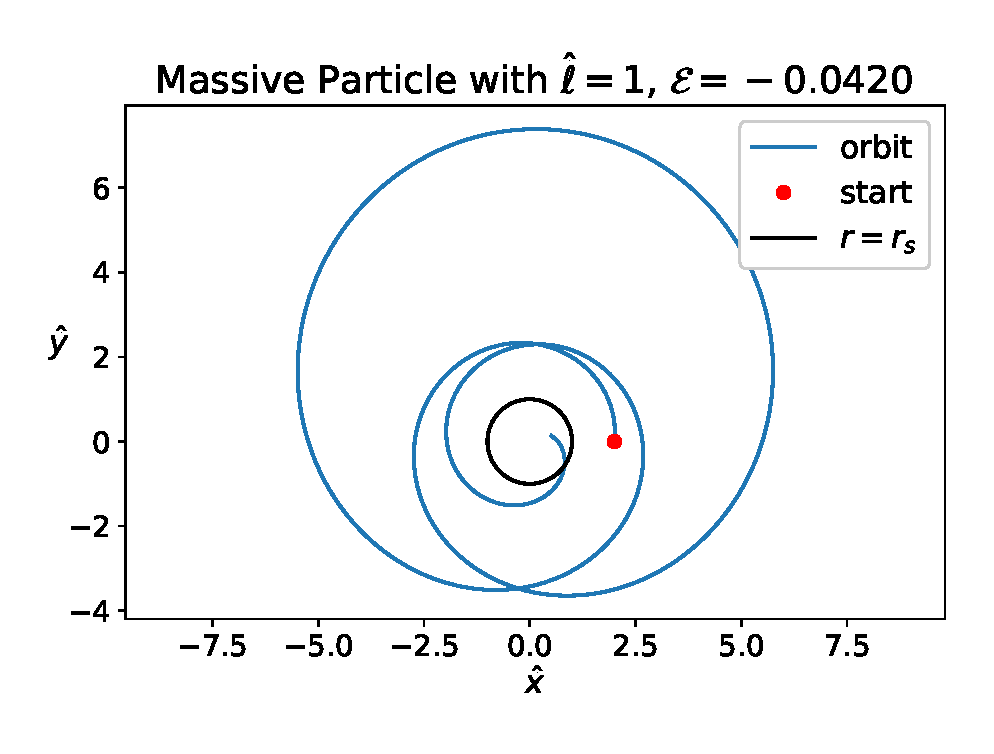
\includegraphics[width=\textwidth]{Figures/chapter2/infall2.eps}
        \caption{$\hat \ell = 1$ and $\mathcal E = -0.042$.
        The particle starts at $\hat r = 2$ with the radial velocity directed
        outwards, but has a negative energy and will not be able to escape.}

    \end{minipage}
\end{figure}




